\documentclass[11pt]{article}
\usepackage[margin=0.5in]{geometry}
\usepackage{cite}
\usepackage{graphicx}
\title{Software methodologies: Image processing: A report on Non-Local Means Denoising}
\author{James Goodall}

\begin{document}
\maketitle
\section{The non-local means denoising algorithm.}

Non-local means is an algorithm for denoising images, based on the principle of replacing a pixel of an mean of all the pixels in the image weighted by how similar their surroundings are to the surroundings of the original pixel. 

As the introduction of \cite{Buades} states, the goal of image denoising methods is to recover the original image from a noisy measurement.

As described in \cite{dip20}, the value of a pixel can be thought of as the sum of the original value plus a random noise element e.g.

\[P = P_0 + N\]

because of this, we can take multiple similar areas in the image we are trying to denoise, each with a different noise added to it but the same original value e.g.

\[P_1 = P_0 + N_1\]
\[P_2 = P_0 + N_2\]
\[\vdots\]
\[P_n = P_0 + N_n\]

finding the mean of $P_n$ results in the sum of $P_0$ and the average of $N$. Since $N$ can be modeled with a mean of $0$, for large values of $n$ the mean of $P_n$ tends towards $P_0$

\subsection{The Algorithm} \label{algorithm}

the algorithm is defined by \cite{Buades_2005} to be: 

\[NL(v)(i) = \sum_{j \in I}{w(i,j)v(j)}\]

with $w(i,j)$ being the similarity function, which is the square of the euclidian distance between the two areas surrounding the pixels i and j, calculated by:

\[\left\|v\left(\mathcal{N}_{i}\right)-v\left(\mathcal{N}_{j}\right)\right\|_{2, a}^{2}\]

with $\mathcal{N}_i$ refering to the pixels surrounding i

A useful property of this similarity function is that, as explained in \cite{Buades_2005} is that the Euckudean distance preserves the order of similarity between pixels, which is to say, that the similarity of $a$ to $b$ is the same as the similarity of $b$ to $a$.

\section{Implementations of the algorithm and their efficiency.}

There are two main implementations of the algorithm, pixelwise and patchwise:

\subsection{Pixelwise}

The pixelwise implemtation is as described in section \ref{algorithm}, howevere due to computational limitations, in \cite{Buades_2011}, the search windows, instead of being the entire image, is limited to a $21\times 21$ square around the pixel in question for small values of $\sigma$ and to a $35 \times 35$ square for large values.

\subsection{Patchwise}

The patchwise implementation of the algorithm is similar to the pixelwise, except that it is applied to a patch instead of a pixel, and the final value of each pixel is the mean value of all the patches it is part of.

The Patchwise implementation has an algorithmic complexity of $N^2(2f + 1)^2$ where f is the patch size.

\section{The influence of the algorithmic parameters on the output.}

\begin{figure}
    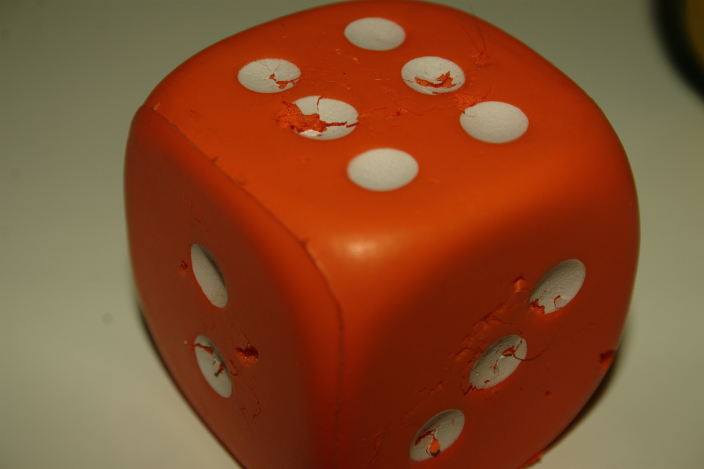
\includegraphics[width=1.75in]{Images/dice.png}
    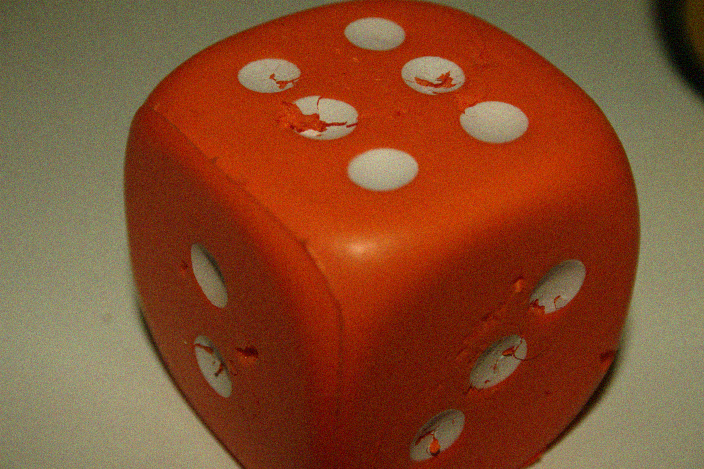
\includegraphics[width=1.75in]{Images/dice-Noise.png}
    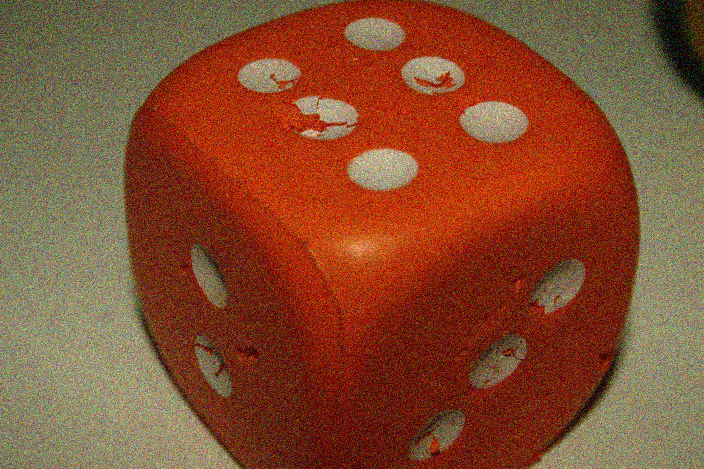
\includegraphics[width=1.75in]{Images/dice-highNoise.png}
    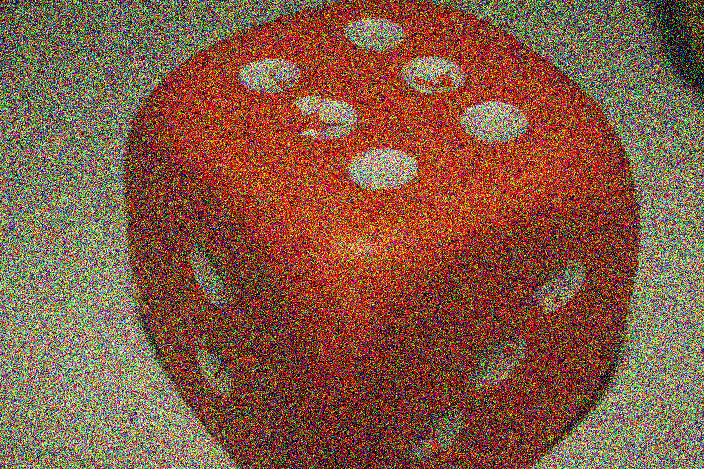
\includegraphics[width=1.75in]{Images/dice-extremeNoise.png}
    \caption{An image of a die, with gradually more noise}
    \label{fig:diceNoiseProgression}
\end{figure}

Figure \ref{fig:diceNoiseProgression} shows the image we are going to use to demonstrate the effects of the algorithms parameters.




\section{The strengths and limitations of non-local means compared to other denoising algorithms. }



\section{Modifications and extensions of the algorithm that have been proposed in the literature. }

An extension of the algorithm that has been proposed in \cite{Tasdizen_2008} is to use principle component analysis (PCA) to significantly reduce the dimentionality of the similarity calculation.

The idea is to model the image neighbourhood as a vector (e.g. for a $7 \times 7$ neighbourhood, 49 dimensions would be used) and find a number of principle components e.g. 6. Then, when comparing the similarities between neighbourhoods, find the Euclidian distance between the values in the 6 principle components for the areas. 

Because the Euclidian distance is calculated between two only 6 dimentional vectors rather than two 49 dimentional vectors, \cite{Tasdizen_2008} finds that the computational cost of the non-local means algorithm is improved upon, and because the dimensions chosen are principle components, this can be achieved without a large loss in quality.

\section{Applications of the original algorithm and its extensions. }


application to video

\bibliography{research}
\bibliographystyle{plain}
\pagebreak
\section{appendix}


\end{document}
